\setcounter{section}{2}
\section{Phương trình mặt cầu}
% \chude{Xác định các yếu tố cơ bản mặt cầu, lập phương trình mặt cầu}
	
\begin{dang}{XÁC ĐỊNH CÁC YẾU TỐ CƠ BẢN MẶT CẦU}
	\begin{itemize}
		\item Phương trình mặt cầu $(S)$ có dạng $(x-a)^2+(y-b)^2+(z-c)^2=R^2$ thì mặt cầu có tâm $I(a;b;c)$ và có bán kính $R$.
		\item Phương trình mặt cầu $(S)$ có dạng $x^2+y^2+z^2-2ax-2by-2cz+d=0$ với $a^2+b^2+c^2-d>0$ thì để xác định tọa độ tâm $I(a;b;c)$ và bán kính $R$ ta thức hiện như sau:
		\begin{itemize}
			\item Xác định tọa độ tâm $I$: $\heva{& -2a=\ldots \\ & -2b=\ldots \\ & -2c=\ldots}$
			\item Xác định bán kính: $R=\sqrt{a^2+b^2+c^2-d}$.
		\end{itemize}
	\end{itemize}
	\begin{note} \textbf{Chú ý:}
		\begin{itemize}
			\item Có thể xác định tọa độ tâm $I(a;b;c)$ và bán kính $R$ của phương trình mặt cầu $(S)$ có dạng $x^2+y^2+z^2-2ax-2by-2cz+d=0$ bằng cách nhóm nhân tử để đưa về dạng $(x-a)^2+(y-b)^2+(z-c)^2=R^2$.
			\item Để một phương trình là một phương trình mặt cầu, cần thỏa mãn hai điều kiện: Hệ số trước $x^2$, $y^2$, $z^2$ phải bằng $1$ và $a^2+b^2+c^2-d>0$.
			\item Nếu $IM=R$ thì $M$ nằm trên mặt cầu.
			\item Nếu $IM<R$ thì $M$ nằm trong mặt cầu.
			\item Nếu $IM>R$ thì $M$ nằm ngoài mặt cầu.
		\end{itemize}
	\end{note}
\end{dang}
\Opensolutionfile{ans}[ans/ans-C5B3CD1_2-11]
\TN

\begin{ex}%[2H5N3-1]
	Cho điểm $M$ nằm ngoài mặt cầu $S(O;R)$. Khẳng định nào dưới đây đúng?
	\choice
	{$OM<R$}
	{$OM=R$}
	{\True $OM>R$}
	{$OM\le R$}
	\loigiai{$M$ nằm ngoài mặt cầu $S(O;R)\Rightarrow OM>R$.}
\end{ex}

\begin{ex}%[2H5N3-2]
	Trong KG $Oxyz$, cho mặt cầu $(S)\colon x^2+(y-2)^2+(z+1)^2=6$. Đường kính của $(S)$ bằng
	\choice
	{$\sqrt{6}$}
	{$12$}
	{\True $2\sqrt{6}$}
	{$3$}
	\loigiai{
		Ta có bán kính của $(S)$ là $\sqrt{6}$ nên đường kính của $(S)$ bằng $2\sqrt{6}$.}
\end{ex}

\begin{ex}%[2H5H3-2]
	Mặt cầu $(S)\colon3x^2+3y^2+3z^2-6x+12y+2=0$ có bán kính bằng
	\choice
	{$\dfrac{\sqrt{7}}{3}$}
	{$\dfrac{2\sqrt{7}}{3}$}
	{$\dfrac{\sqrt{21}}{3}$}
	{\True $\sqrt{\dfrac{13}{3}}$}
	\loigiai{
		Ta có $3x^2+3y^2+3z^2-6x+12y+2=0\Leftrightarrow  x^2+y^2+z^2-2x+4y+\dfrac{2}{3}=0$.\\
		Do đó mặt cầu $(S)$ có tâm $I\left(1;-2;0\right)$, bán kính $R=\sqrt{\dfrac{13}{3}}$.}
\end{ex}

\begin{ex}%[2H5N3-2]
	Trong KG $Oxyz$, cho mặt cầu $(S)\colon(x-2)^2+(y+1)^2+(z-3)^2=4$. Tâm của $(S)$ có tọa độ là
	\choice
	{$(-2;1;-3)$}
	{$(-4;2;-6)$}
	{$(4;-2;6)$}
	{\True $(2;-1;3)$}
	\loigiai{
		Mặt cầu $(S)\colon (x-2)^2+(y+1)^2+(z-3)^2=4$ có tâm $I(2;-1;3)$.}
\end{ex}

\begin{ex}%[2H5N3-2]
	Trong KG $Oxyz$, mặt cầu $(S)\colon (x+1)^2+(y-2)^2+z^2=9$ có bán kính bằng
	\choice
	{\True $3$}
	{$81$}
	{$9$}
	{$6$}
	\loigiai{Mặt cầu $(S)$ có bán kính $R=3$.}
\end{ex}
	
\begin{ex}%[2H5N3-3]
	Trong KG $Oxyz$, cho mặt cầu $(S)$ có tâm $I(1;-4;0)$ và bán kính bằng $3$. Phương trình của $(S)$ là
	\choice
	{$(x+1)^2+(y-4)^2+z^2=9$}
	{$(x-1)^2+(y+4)^2+z^2=9$}
	{\True $(x-1)^2+(y+4)^2+z^2=9$}
	{$(x+1)^2+(y-4)^2+z^2=3$}
	\loigiai{
		Mặt cầu $(S)$ có tâm $I(1;-4;0)$ có bán kính $3$ có phương trình là $(x-1)^2+(y+4)^2+z^2=9$.}
\end{ex}	
	
\begin{ex}%[2H5N3-2]
	Trong KG $Oxyz$, cho mặt cầu $(S)\colon x^2+y^2+(z-1)^2=16$. Bán kính của $(S)$ là
	\choice
	{$32$}
	{$8$}
	{$4$}
	{$16$}
	\loigiai{
		Từ phương trình mặt cầu $(S)\colon x^2+y^2+(z-1)^2=16\Rightarrow$ bán kính $R=\sqrt{16}=4$.}
\end{ex}	
	
\begin{ex}%[2H5N3-2]
	Trong KG $Oxyz$, cho mặt cầu $(S)\colon (x+1)^2+(y+2)^2+(z-3)^2=9$. Tâm của $(S)$ có tọa độ là
	\choice
	{$(-2;-4;6)$}
	{$(2;4;-6)$}
	{\True $(-1;-2;3)$}
	{$(1;2;-3)$}
	\loigiai{
		Tâm của $(S)$ có tọa độ là $(-1;-2;3)$.}
\end{ex}
	
\begin{ex}%[2H5H3-2]
	Trong KG $Oxyz$, cho mặt cầu $(S)\colon x^2+y^2+z^2-8x+10y-6z+49=0$. Tính bán kính $R$ của mặt cầu $(S)$.
	\choice
	{\True $R=1$}
	{$R=7$}
	{$R=\sqrt{151}$}
	{$R=\sqrt{99}$}
	\loigiai{
		Ta có $a=4$, $b=-5$, $c=3$, $d=49$. Do đó $R=\sqrt{a^2+b^2+c^2-d}=1$.}
\end{ex}
		
\begin{ex}%[2H5N3-2]
	Trong KG $Oxyz$, cho mặt cầu có phương trình $(x-1)^2+(y+2)^2+(z-3)^2=4$. Tìm tọa độ tâm $I$ và bán kính $R$ của mặt cầu đó.
	\choice
	{$I(-1;2;-3)$; $R=2$}
	{$I(-1;2;-3)$; $R=4$}
	{\True $I(1;-2;3)$; $R=2$}
	{$I(1;-2;3)$; $R=4$}
	\loigiai{
		Mặt cầu đã cho có tâm $I\left(1;-2;3\right)$ và bán kính $R=2$.}
\end{ex}		
		
\begin{ex}%[2H5H3-2]
	Trong KG $Oxyz$, trong các mặt cầu dưới đây, mặt cầu nào có bán kính $R=2$?
	\choice
	{$(S)\colon x^2+y^2+z^2-4x+2y+2z-3=0$}
	{$(S)\colon x^2+y^2+z^2-4x+2y+2z-10=0$}
	{\True $(S)\colon x^2+y^2+z^2-4x+2y+2z+2=0$}
	{$(S)\colon x^2+y^2+z^2-4x+2y+2z+5=0$}
	\loigiai{
		Ta có mặt cầu $(S)\colon x^2+y^2+z^2-2ax-2by-2cz+d=0$ có bán kính là $R=\sqrt{a^2+b^2+c^2-d}$.\\
		Với $(S)\colon x^2+y^2+z^2-4x+2y+2z+2=0$, ta có $\heva{
			& a=2\\ 
			& b=-1\\ 
			& c=-1\\ 
			& d=2.}$\\
	Suy ra $R=\sqrt{a^2+b^2+c^2-d}=\sqrt{4}=2$.}
\end{ex}
		
\begin{ex}%[2H5H3-3]
	Cho các phương trình sau
	\begin{listEX}[2]
		\item $\left(x-1\right)^2+y^2+z^2=1$;
		\item $x^2+\left(2y-1\right)^2+z^2=4$;
		\item $x^2+y^2+z^2+1=0$;
		\item $\left(2x+1\right)^2+\left(2y-1\right)^2+4z^2=16$.
	\end{listEX}
	Số phương trình là phương trình mặt cầu là
	\choice
	{$4$}
	{$3$}
	{\True $2$}
	{$1$}
	\loigiai{
		Ta có $\left(2x+1\right)^2+\left(2y-1\right)^2+4z^2=16\Leftrightarrow{\left(x+\dfrac{1}{2}\right)^2}+\left(y-\dfrac{1}{2}\right)^2+z^2=4$ là phương trình mặt cầu.\\
		$\left(x-1\right)^2+y^2+z^2=1$ là phương trình của một mặt cầu.}
\end{ex}
		
\begin{ex}%[2H5H3-2]
	Trong không gian với hệ trục tọa độ $Oxyz$, gọi $I$ là tâm mặt cầu $(S)\colon x^2+y^2+(z-2)^2=4$. Độ dài $\left|\overrightarrow{OI}\right|$ bằng
	\choice
	{\True $2$}
	{$4$}
	{$1$}
	{$\sqrt{2}$}
	\loigiai{
		Mặt cầu $(S)$ có tâm $I(0;0;2)\Rightarrow\overrightarrow{OI}=(0;0;2)\Rightarrow\left|\overrightarrow{OI}\right|=2$.}
\end{ex}
			
\begin{ex}%[2H5H3-3]
	Trong KG $Oxyz$ có tất cả bao nhiêu giá trị nguyên $m$ để phương trình $x^2+y^2+z^2+4mx+2my-2mz+9m^2-28=0$ là phương trình mặt cầu?
	\choice
	{\True $7$}
	{$8$}
	{$9$}
	{$6$}
	\loigiai{
		Ta có 
		$$\begin{aligned}
			&x^2+y^2+z^2+4mx+2my-2mz+9m^2-28=0\\
			\Leftrightarrow\ &(x+2m)^2+(y+m)^2+(z-m)^2=28-3m^2.\quad(1)
		\end{aligned}$$
		$(1)$ là phương trình mặt cầu $\Leftrightarrow 28-3m^2>0\Leftrightarrow-\sqrt{\dfrac{28}{3}}<m<\sqrt{\dfrac{28}{3}}$.\\
		Do $m$ nguyên nên $m\in\left\{-3;-2;-1;0;1;2;3\right\}$.\\
		Vậy có $7$ giá trị của $m$ thỏa mãn yêu cầu bài toán.}
\end{ex}			
				
\begin{ex}%[2H5H3-3]
	Trong KG $Oxyz$, có tất cả bao nhiêu giá nguyên của $m$ để
	$x^2+y^2+z^2+2\left(m+2\right)x-2\left(m-1\right)z+3m^2-5=0$ là phương trình một mặt cầu?
	\choice
	{$4$}
	{$6$}
	{$5$}
	{\True $7$}
\loigiai{
	Phương trình đã cho là phương trình mặt cầu khi và chỉ khi
	$$\begin{aligned}
		(m+2)^2+(m-1)^2-3m^2+5>0 
		&\Leftrightarrow m^2-2m-10<0\\ 
		&\Leftrightarrow-1-\sqrt{11}<m<1+\sqrt{11}.
	\end{aligned}$$
	Vì $m\in\mathbb{Z}\Rightarrow m=\{-2;-1;0;1;2;3;4\}\Rightarrow $ có $7$ giá trị của $m$ nguyên thỏa mãn bài toán.}
\end{ex}	

\begin{ex}%[2H5H3-3]
	Cho phương trình $x^2+y^2+z^2-4x+2my+3m^2-2m=0$ với $m$ là tham số. Tính tổng tất cả các giá trị nguyên của $m$ để phương trình đã cho là phương trình mặt cầu.
	\choice
	{$0$}
	{\True $1$}
	{$2$}
	{$3$}
	\loigiai{
		Giả sử $x^2+y^2+z^2-4x+2my+3m^2-2m=0$ là phương trình mặt cầu.\\
		Khi đó tâm mặt cầu là $I(2;-m;0)$, và bán kính $$R=\sqrt{4+m^2-\left(3m^2-2m\right)}=\sqrt{-2m^2+2m+4} \text{ với }-2m^2+2m+4>0\Leftrightarrow m\in(-1;2).$$
		Do $m\in\mathbb{Z}\Rightarrow m\in\{ 0;1\}$.\\
		Vậy tổng tất cả các giá trị nguyên của $m$ bằng $1$.}
\end{ex}

\Closesolutionfile{ans}
% \indapan{10}{ans/ans-C5B3CD1_2-11}		
\TNTF
\Opensolutionfile{ans}[ans/ans-C5B3CD1_2-11-DS]

\begin{ex}%[2H5N3-2]
	Trong KG $Oxyz$, cho mặt cầu $(S)\colon x^2+y^2+(z+2)^2=9$ có tâm $I$ và bán kính $R$. Các mệnh đề sau đây đúng hay sai?
	\choiceTF
	{Tọa độ tâm mặt cầu $(S)$ là $I(0;0;2)$}
	{Bán kính mặt cầu $(S)$ là $R=9$}
	{\True Khoảng cách từ tâm mặt cầu đến mặt phẳng $(P)\colon x+y+z=0$ bằng $\dfrac{2\sqrt{3}}{3}$}
	{\True Diện tích mặt cầu $(S)$ bằng $36\pi$}
	\loigiai{
		\begin{itemchoice}
			\itemch \textbf{Sai.} Tọa độ tâm mặt cầu là $I\left(0;0;-2\right)$.
			\itemch \textbf{Sai.} Bán kính của mặt cầu là $R=3$.
			\itemch \textbf{Đúng.} Ta có $\mathrm{d}(I,(P))=\dfrac{|0+0+2|}{\sqrt{1^2+1^2+1^2}}=\dfrac{2\sqrt{3}}{3}$.
			\itemch \textbf{Đúng.} Diện tích mặt cầu $S=4\pi R^2=4\pi\cdot 3^2=36\pi$.
		\end{itemchoice}
		}
\end{ex}

\begin{ex}%[2H5H3-2]
	Trong KG $Oxyz$, cho mặt cầu $(S)\colon(x+3)^2+y^2+(z-2)^2=16$ có tâm $I$ và bán kính $R$. Các mệnh đề sau đây đúng hay sai?
	\choiceTF
	{\True Điểm $M(-1;0;3)$ nằm trong mặt cầu $(S)$}
	{\True Bán kính mặt cầu $(S)$ là $R=4$}
	{\True Tọa độ tâm mặt cầu $(S)$ là $I(-3;0;2)$}
	{Thể tích mặt cầu $(S)$ là $V=\dfrac{16384\pi}{3}$}
	\loigiai{
		\begin{itemchoice}
			\itemch \textbf{Đúng.} Thay tọa độ điểm $M$ vào vế trái của phương trình $(S)$ ta có $$(-1+3)^2+0^2+(3-2)^2=5<16.$$
			Suy ra $M$ nằm trong mặt cầu $(S)$.
			\itemch \textbf{Đúng.} Bán kính mặt cầu là $R=4$.
			\itemch \textbf{Đúng.} Tọa độ tâm mặt cầu là $I(-3;0;2)$.
			\itemch \textbf{Sai.} Thể tích mặt cầu $(S)$ là $V=\dfrac{256\pi}{3}$.
		\end{itemchoice}
		}
\end{ex}

\begin{ex}%[2H5H3-2]
	Trong không gian với hệ toạ độ $Oxyz$, cho điểm $M(2;0;2)$ và mặt cầu $(S)\colon x^2+(y+2)^2+(z-2)^2=8$. Các mệnh đề sau đây đúng hay sai?
	\choiceTF
	{\True Điểm $M\left(2;0;2\right)$ thuộc mặt cầu $(S)$}
	{\True Bán kính mặt cầu $(S)$ là $R=2\sqrt{2}$}
	{\True Tọa độ tâm mặt cầu $(S)$ là $I\left(0;-2;2\right)$}
	{Hình chiếu của tâm mặt cầu lên trục $Ox$ là điểm có tọa độ $(0;0;2)$}
	\loigiai{
		\begin{itemchoice}
			\itemch \textbf{Đúng.} Thay tọa độ điểm $M\left(2;0;2\right)$ vào mặt cầu, ta có $2^2+2^2+(2-2)^2=8\Rightarrow M(2;0;2)\in(S)$.
			\itemch \textbf{Đúng.} Mặt cầu $(S)$ có bán kính $R=2\sqrt{2}$.
			\itemch \textbf{Đúng.} Mặt cầu $(S)$ có tâm $I(0;-2;2)$.
			\itemch \textbf{Sai.} Hình chiếu của tâm mặt cầu lên trục $Ox$ là $O(0;0;0)$.
		\end{itemchoice}
		}
\end{ex}

\begin{ex}%[2H5N3-2]
	Trong KG $Oxyz$, mặt cầu $(S)\colon(x-1)^2+(y+2)^2+(z-4)^2=20$. Các mệnh đề sau đây đúng hay sai?
	\choiceTF
	{Bán kính mặt cầu $(S)$ là $20$}
	{Diện tích mặt cầu $(S)$ là $1600\pi$}
	{Tọa độ tâm mặt cầu $(S)$ là $I\left(-1;2;-4\right)$}
	{\True Điểm đối xứng của tâm mặt cầu $(S)$ qua mặt phẳng $(Oyz)$ là $I\left(-1;-2;4\right)$}
	\loigiai{
		\begin{itemchoice}
			\itemch \textbf{Sai.} Mặt cầu $(x-1)^2+(y+2)^2+(z-4)^2=20$ có bán kính là $R=2\sqrt{5}$.
			\itemch \textbf{Sai.} Diện tích mặt cầu $(S)$ bằng $S=4\pi R^2=4\pi \left(2\sqrt{5}\right)^2=80\pi$.
			\itemch \textbf{Sai.} Mặt cầu $(x-1)^2+(y+2)^2+(z-4)^2=20$ có tâm là $I(1;-2;4)$.
			\itemch \textbf{Đúng.} Điểm đối xứng của tâm $I(1;-2;4)$ của mặt cầu $(S)$ qua mặt phẳng $(Oyz)$ là $I\left(-1;-2;4\right)$.
		\end{itemchoice}
		}
\end{ex}

\begin{ex}%[2H5H3-3]
	Trong KG $Oxyz$, cho các phương trình sau
	\begin{listEX}
		\item $(S_1)\colon x^2+y^2+z^2+x-2y+4z-3=0$, 
		\item $(S_2)\colon 2x^2+2y^2+2z^2-x-y-z=0$,
		\item $(S_3)\colon 2x^2+2y^2+2z^2+4x+8y+6z+3=0$, 
		\item $(S_4)\colon x^2+y^2+z^2-2x+4y-4z+10=0$.
	\end{listEX}
	Các mệnh đề sau đây đúng hay sai?
	\choiceTF
	{\True $(S_1)$ là phương trình của một mặt cầu}
	{\True $(S_2)$ là phương trình của một mặt cầu}
	{$(S_3)$ không phải là phương trình của một mặt cầu}
	{\True $(S_4)$ không phải là phương trình của một mặt cầu}
	\loigiai{
		 Phương trình $x^2+y^2+z^2-2ax-2by-2cz+d=0$ là phương trình của một mặt cầu nếu $a^2+b^2+c^2-d>0$.
		\begin{itemchoice}
			\itemch \textbf{Đúng.}
			$(S_1)\colon x^2+y^2+z^2+x-2y+4z-3=0\Rightarrow \heva{
				& a=-\dfrac{1}{2}\\ 
				& b=1\\ 
				& c=-2\\ 
				& d=-1}\Rightarrow a^2+b^2+c^2-d>0$.
			\itemch \textbf{Đúng.} $(S_2)\colon 2x^2+2y^2+2z^2-x-y-z=0\Leftrightarrow x^2+y^2+z^2-\dfrac{1}{2}x-\dfrac{1}{2}y-\dfrac{1}{2}z=0$.\\
			Suy ra $\heva{
				& a=\dfrac{1}{4}\\ 
				& b=\dfrac{1}{4}\\ 
				& c=\dfrac{1}{4}\\ 
				& d=0}\Rightarrow a^2+b^2+c^2-d>0$.
			\itemch \textbf{Sai.} $(S_3)\colon 2x^2+2y^2+2z^2+4x+8y+6z+3=0\Leftrightarrow x^2+y^2+z^2+2x+4y+3z+\dfrac{3}{2}=0$.\\
			Suy ra $\heva{
				& a=-1\\ 
				& b=-2\\ 
				& c=-\dfrac{3}{2}\\ 
				& d=\dfrac{3}{2}}\Rightarrow a^2+b^2+c^2-d>0$.
			\itemch \textbf{Đúng.} $(S_4)\colon x^2+y^2+z^2-2x+4y-4z+10=0 \Rightarrow\heva{
				& a=1\\ 
				& b=-2\\ 
				& c=2\\ 
				& d=10}\Rightarrow a^2+b^2+c^2-d<0$.
		\end{itemchoice}
		}
\end{ex}

\begin{ex}%[2H5H3-3]
	Trong KG $Oxyz$, cho các phương trình sau
	\begin{listEX}[2]
		\item $(S_1)\colon x^2+y^2+z^2-2x=0$, 
		\item $(S_2)\colon x^2+y^2-z^2+2x-y+1=0$,
		\item $(S_3)\colon 2x^2+2y^2=(x+y)^2-z^2+2x-1$,
		\item $(S_4)\colon (x+y)^2=2xy-z^2-1$.
	\end{listEX}
	Các mệnh đề sau đây đúng hay sai?
	\choiceTF
	{\True $(S_1)$ là phương trình của một mặt cầu}
	{$(S_2)$ là phương trình của một mặt cầu}
	{$(S_3)$ là phương trình của một mặt cầu}
	{\True $(S_4)$ không phải là phương trình của một mặt cầu}
	\loigiai{
		Phương trình mặt cầu $(S)$ có hai dạng là\\
		(1) $(x-a)^2+(y-b)^2+(z-c)^2=R^2$;\\
		(2) $x^2+y^2+z^2-2ax-2by-2cz+d=0$ với $a^2+b^2+c^2-d>0$.
		\begin{itemchoice}
			\itemch \textbf{Đúng.} Ta có $(S_1)\colon x^2+y^2+z^2-2x=0\Leftrightarrow (x-1)^2+y^2+z^2=1$.\\
			Do đó $(S_1)$ là phương trình mặt cầu.
			\itemch \textbf{Sai.} Ta có $(S_2)$ không là phương trình mặt cầu vì các hệ số của $x^2$, $y^2$, $z^2$ không bằng nhau.
			\itemch \textbf{Sai.} Ta có $(S_3)\colon 2x^2+2y^2=(x+y)^2-z^2+2x-1\Leftrightarrow x^2+y^2+z^2-2xy-2x+1=0$.\\
			Vì phương trình có chứa $xy$ nên $(S_3)$ không phải phương trình mặt cầu.
			\itemch \textbf{Đúng.} Ta có $(S_4)\colon (x+y)^2=2xy-z^2-1\Leftrightarrow x^2+y^2+z^2=1$.\\
			Do đó $(S_4)$ là phương trình mặt cầu.
		\end{itemchoice}
		}
\end{ex}

\begin{ex}%[2H5H3-3]
	Trong KG $Oxyz$, cho các phương trình sau
	\begin{listEX}[2]
		\item $(S_1)\colon x^2+y^2+z^2-2x=0$,
		\item $(S_2)\colon 2x^2+2y^2=(x+y)^2-z^2+2x-1$,
		\item $(S_3)\colon x^2+y^2+z^2+2x-2y+1=0$,
		\item $(S_4)\colon (x+y)^2=2xy-z^2+1-4x$.
	\end{listEX}
	Các mệnh đề sau đây đúng hay sai?
	\choiceTF
	{\True $(S_1)$ là phương trình của một mặt cầu}
	{$(S_2)$ là phương trình của một mặt cầu}
	{\True $(S_3)$ là phương trình của một mặt cầu}
	{\True $(S_4)$ là phương trình của một mặt cầu}
	\loigiai{
		Phương trình mặt cầu $(S)$ có hai dạng là\\
		(1) $(x-a)^2+(y-b)^2+(z-c)^2=R^2$;\\
		(2) $x^2+y^2+z^2-2ax-2by-2cz+d=0$ với $a^2+b^2+c^2-d>0$.
		\begin{itemchoice}
			\itemch \textbf{Đúng.} Ta có $(S_1)\colon x^2+y^2+z^2-2x=0\Leftrightarrow (x-1)^2+y^2+z^2=1$.\\
			Do đó $(S_1)$ là phương trình mặt cầu.
			\itemch \textbf{Sai.} Ta có $(S_2)\colon 2x^2+2y^2=(x+y)^2-z^2+2x-1\Leftrightarrow x^2+y^2+z^2-2xy-2x+1=0$.\\
			Vì phương trình có chứa $xy$ nên $(S_2)$ không phải phương trình mặt cầu.
			\itemch \textbf{Đúng.} Ta có $(S_3)\colon x^2+y^2+z^2+2x-2y+1=0\Leftrightarrow (x+1)^2+(y-1)^2+z^2=1$.\\
			Do đó $(S_3)$ là phương trình mặt cầu.
			\itemch \textbf{Đúng.} Ta có $(S_4)\colon (x+y)^2=2xy-z^2+1-4x\Leftrightarrow (x+2)^2+y^2+z^2=5$.\\
			Do đó $(S_4)$ là phương trình mặt cầu.
		\end{itemchoice}
		}
\end{ex}

\begin{ex}%[2H5H3-3]
	Trong KG $Oxyz$, cho các phương trình sau
	\begin{listEX}[2]
		\item $(S_1)\colon (x-1)^2+(2y-1)^2+(z-1)^2=6$, 
		\item $(S_2)\colon (x-1)^2+(y-1)^2+(z-1)^2=6$,
		\item $(S_3)\colon (2x-1)^2+(2y-1)^2+(2z+1)^2=6$,
		\item $(S_4)\colon (x+y)^2=2xy-z^2+3-6x$.
	\end{listEX}
	Các mệnh đề sau đây đúng hay sai?
	\choiceTF
	{\True $(S_1)$ không phải là phương trình của một mặt cầu}
	{$(S_2)$ không phải là phương trình của một mặt cầu}
	{$(S_3)$ không phải là phương trình của một mặt cầu}
	{$(S_4)$ không phải là phương trình của một mặt cầu}
	\loigiai{
		Phương trình mặt cầu $(S)$ có hai dạng là\\
		(1) $(x-a)^2+(y-b)^2+(z-c)^2=R^2$;\\
		(2) $x^2+y^2+z^2-2ax-2by-2cz+d=0$ với $a^2+b^2+c^2-d>0$.
		\begin{itemchoice}
			\itemch \textbf{Đúng.} Ta có hệ số của $x$, $y$, $z$ trong phương trình không bằng nhau nên $(S_1)$ không phải là phương trình của một mặt cầu.
			\itemch \textbf{Sai.} Vì $(S_2)\colon (x-1)^2+(y-1)^2+(z-1)^2=6$ là phương trình mặt cầu.
			\itemch \textbf{Sai.} Vì $$(S_3)\colon (2x-1)^2+(2y-1)^2+(2z+1)^2=6\Leftrightarrow \left(x-\dfrac{1}{2}\right)^2+\left(y-\dfrac{1}{2}\right)^2+\left(z+\dfrac{1}{2}\right)^2=\dfrac{3}{2}.$$
			Do đó $(S_3)$ là phương trình mặt cầu.
			\itemch \textbf{Sai.} $(S_4)\colon (x+y)^2=2xy-z^2+3-6x\Leftrightarrow (x+3)^2+y^2+z^2=12.$\\
			Do đó $(S_4)$ là phương trình mặt cầu.
		\end{itemchoice}
		}
\end{ex}

\begin{ex}%[2H5H3-3]
	Trong không gian với hệ trục $Oxyz$, cho phương trình $(S)\colon x^2+y^2+z^2-2(m+2)x+4my-2mz+5m^2+9=0$. Các mệnh đề sau đây đúng hay sai?
	\choiceTF
	{Với $m=0$ thì $(S)$ là phương trình của một mặt cầu}
	{Với $m=1$ thì $(S)$ là phương trình của một mặt cầu có tâm $I(3;-2;1)$}
	{\True Với $m=3$ thì $(S)$ là phương trình của một mặt cầu có bán kính là $R=4$}
	{\True Với $m<-5$ hoặc $m>1$ thì $(S)$ là phương trình của một mặt cầu}
\loigiai{
	
	\begin{itemchoice}
		\itemch \textbf{Sai.} Với $m=0$, ta có $\heva{&a=2\\&b=0\\&c=0\\&d=9}$. Khi đó $a^2+b^2+c^2-d=-5<0$. \\
		Suy ra $(S)$ không là phương trình mặt cầu.
		\itemch \textbf{Sai.} Với $m=1$, ta có $\heva{&a=3\\&b=-2\\&c=1\\&d=14}$. Khi đó $a^2+b^2+c^2-d=0$. \\
		Suy ra $(S)$ không là phương trình mặt cầu.
		\itemch \textbf{Đúng.} Với $m=3$, ta có $\heva{&a=5\\&b=-6\\&c=3\\&d=54}$. Khi đó $a^2+b^2+c^2-d=16>0$. \\
		Suy ra $(S)$ là phương trình mặt cầu có bán kính $R=\sqrt{a^2+b^2+c^2-d}=4$.
		\itemch \textbf{Đúng.} Ta có điều kiện xác định mặt cầu là $a^2+b^2+c^2-d>0$, khi đó
		$$\left(m+2\right)^2+4m^2+m^2-5m^2-9>0\Leftrightarrow m^2+4m-5>0\Leftrightarrow\hoac{
			& m<-5\\ 
			& m>1.}$$
	\end{itemchoice}
	}
\end{ex}

\Closesolutionfile{ans}
% \indapan{3}{ans/ans-C5B3CD1_2-11-DS}

\Opensolutionfile{ans}[ans/ans-C5B3CD1_2-11-KQ]
\TNSA
\begin{ex}%[2H5N3-2]
	Trong KG $Oxyz$, cho mặt cầu $(S)\colon (x-1)^2+(y+2)^2+(z-3)^2=16$. Tọa độ tâm của mặt cầu $(S)$ là $(a;b;c)$. Khi đó $a+b+c$ bằng bao nhiêu?
	\shortans{$2$}
	\loigiai{
	Mặt cầu $(S)\colon (x-1)^2+(y+2)^2+(z-3)^2=16$ có tâm là $I(1;-2;3)$.\\
	Suy ra $a=1$, $b=-2$, $c=3$. Khi đó $a+b+c=2$.
	}
\end{ex}
\begin{ex}%[2H5H3-2]
	Trong không gian với hệ trục tọa độ $Oxyz$, tất cả các giá trị của $m$ để phương trình $x^2+y^2+z^2-2(m+2)x+4my+19m-6=0$ là phương trình mặt cầu là $S=(-\infty;a)\cup(b;+\infty)$. Giá trị $a+b$ bằng
	\shortans{$3$}
	\loigiai{
		Điều kiện để phương trình $x^2+y^2+z^2-2(m+2)x+4my+19m-6=0$ là phương trình mặt cầu là $(m+2)^2+4m^2-19m+6>0\Leftrightarrow 5m^2-15m+10>0\Leftrightarrow m<1$ hoặc $m>2$.\\
		Vậy $a=1$ và $b=2$ nên $a+b=3$.
	}
\end{ex}
\begin{ex}%[2H5H3-2]
	Trong không gian với hệ trục tọa độ $Oxyz$, có bao nhiêu giá trị nguyên của $m$ để phương trình $x^2+y^2+z^2+2x-4y+2(m+1)z+2m^2+6=0$ là phương trình mặt cầu.
	\shortans{$1$}
	\loigiai{
		Điều kiện để phương trình $x^2+y^2+z^2+2x-4y+2(m+1)z+2m^2+6=0$ là phương trình mặt cầu là $1^2+(-2)^2+(m+1)^2-2m^2-6>0\Leftrightarrow -m^2+2m>0\Leftrightarrow -2<m<0$.\\
		Vậy có $1$ giá trị nguyên của $m$ thỏa yêu cầu bài toán.
	}
\end{ex}
\begin{ex}%[2H5H3-2]
	Trong không gian với hệ trục tọa độ $Oxyz$, có bao nhiêu giá trị nguyên dương của $m$ để phương trình $x^2+y^2+z^2-2(m+2)x+4my-2mz+5m^2+9=0$ không phải là phương trình mặt cầu.
	\shortans{$1$}
	\loigiai{
		Điều kiện để phương trình $x^2+y^2+z^2-2(m+2)x+4my-2mz+5m^2+9=0$ không là phương trình mặt cầu là $$(m+2)^2+4m^2+m^2-5m^2-9\leq0\Leftrightarrow m^2+4m-5\leq0\Leftrightarrow -5\leq m\leq1.$$
		Vậy có $1$ giá trị nguyên dương $m$ thỏa yêu cầu.
	}
\end{ex}
\begin{ex}%[2H5H3-2]
	Trong không gian với hệ trục tọa độ $Oxyz$, có bao nhiêu giá trị nguyên của $m$ để phương trình $x^2+y^2+z^2-2(3-m)x-2(m+1)y-2mz+2m^2+7=0$ không phải là phương trình mặt cầu.
	\shortans{$3$}
	\loigiai{
		Điều kiện để phương trình $x^2+y^2+z^2-2(3-m)x-2(m+1)y-2mz+2m^2+7=0$ không là phương trình mặt cầu là $$(3-m)^2+(m+1)^2+m^2-2m^2-7\leq0\Leftrightarrow m^2-4m+3\leq0\Leftrightarrow 1\leq m\leq3.$$
		Vậy có $3$ giá trị nguyên $m$ thỏa yêu cầu.
	}
\end{ex}
\begin{ex}%[2H5H3-2]
	Trong KG $Oxyz$, cho hai điểm $A(1;2;1)$, $B(3;1;-2)$. Tập hợp điểm $M(x;y;z)$ sao cho thỏa mãn $MA^2+MB^2=30$ là phương trình mặt cầu tâm $I(a;b;c)$. Giá trị $a+b+c$ bằng
	\shortans{$3$}
	\loigiai{
		Ta có 
		\begin{eqnarray*}
			MA^2+MB^2=30&\Leftrightarrow& (x-1)^2+(y-2)^2+(z-1)^2+(x-3)^2+(y-1)^2+(z+2)^2=30\\
			&\Leftrightarrow& x^2+y^2+z^2-4x-3y+z-5=0.
		\end{eqnarray*}
		Do đó $I\left(2;\dfrac{3}{2};-\dfrac{1}{2}\right)$ suy ra $a+b+c=3$.
	}
\end{ex}
\begin{ex}%[2H5H3-2]
	Trong KG $Oxyz$, cho hai điểm $A(1;2;1)$, $B(3;1;-2)$. Tập hợp điểm $M(x;y;z)$ sao cho thỏa mãn $\dfrac{MB}{MA}=2$ là phương trình mặt cầu tâm $I(a;b;c)$. Giá trị $a+b+c$ gần bằng
	\shortans{$4{,}67$}
	\loigiai{
		Ta có 
		\begin{eqnarray*}
			\dfrac{MB}{MA}=2&\Leftrightarrow&4MA^2=MB^2\\
			&\Leftrightarrow&4(x-1)^2+4(y-2)^2+4(z-1)^2=(x-3)^2+(y-1)^2+(z+2)^2
			\\
			&\Leftrightarrow&x^2+y^2+z^2-\dfrac{2}{3}x-\dfrac{14}{3}y-4z+\dfrac{10}{3}=0.
		\end{eqnarray*}
		Suy ra tâm $I\left(\dfrac{1}{3};\dfrac{7}{3};2\right)$.\\
		Vậy $a+b+c=\dfrac{14}{3}\approx4{,}67$.
	}
\end{ex}
\begin{ex}%[2H5H1-3]
	Trong KG $Oxyz$, cho hai điểm $A(-1;2;0)$, $B(0;1;-2)$. Tập hợp điểm $M(x;y;z)$ sao cho thỏa mãn $MA=MB$ là mặt phẳng có phương trình $x+ay+bz+c=0$. Giá trị $a+b+c$ bằng
	\shortans{$-3$}
	\loigiai{
		Ta có 
		\begin{eqnarray*}
			MA=MB&\Leftrightarrow&(x+1)^2+(y-2)^2+z^2=x^2+(y-1)^2+(z+2)^2\\
			&\Leftrightarrow&x-y-2z=0.
		\end{eqnarray*}
		Vậy $a=-1$, $b=-2$, $c=0$ suy ra $a+b+c=-3$.
	}
\end{ex}
\begin{ex}%[2H5H3-2]
	Trong KG $Oxyz$, cho hai điểm $A(-1;0;1)$, $B(1;-1;2)$. Tập hợp điểm $M(x;y;z)$ sao cho thỏa mãn $\widehat{AMB}=90^\circ$ là mặt cầu tâm $I(a;b;c)$ và bán kính $R=\sqrt{d}$. Giá trị $a+b+c+d$ bằng
	\shortans{$2{,}5$}
	\loigiai{
		Tập hợp điểm $M(x;y;z)$ sao cho thỏa mãn $\widehat{AMB}=90^\circ$ là mặt cầu đường kính $AB$.\\
		Gọi $I$ là trung điểm $AB$ suy ra $I\left(0;-\dfrac{1}{2};\dfrac{3}{2}\right)$ là tâm mặt cầu.\\
		Mặt khác $R=IA=\dfrac{\sqrt{6}}{2}$ suy ra phương trình mặt cầu $x^2+\left(y+\dfrac{1}{2}\right)^2+\left(z-\dfrac{3}{2}\right)^2=\dfrac{3}{2}$.\\
		Do đó $a=0$; $b=-\dfrac{1}{2}$; $c=\dfrac{3}{2}$ và $d=\dfrac{3}{2}$.\\
		Vậy $a+b+c+d=2{,}5$.
		
	}
\end{ex}
\Closesolutionfile{ans}
% \indapan{6}{ans/ans-C5B3CD1_2-11-KQ}
\begin{dang}{LẬP PHƯƠNG TRÌNH MẶT CẦU DẠNG CƠ BẢN}
	Mặt cầu tâm $I(a;b;c)$ và có bán kính $R$ có phương trình $$(S)\colon{(x-a)^2}+(y-b)^2+(z-c)^2=R^2.$$	
	Phương trình $x^2+y^2+z^2-2ax-2by-2cz+d=0$ với $a^2+b^2+c^2-d>0$ là phương trình của mặt cầu tâm $I(a;b;c)$ và bán kính $R=\sqrt{a^2+b^2+c^2-d}$.	
\end{dang}
\TN
\Opensolutionfile{ans}[ans/ans-2-C5-B3-CD1-D2-LC]
%%==========Câu 1
\begin{ex}%[2H5N3-3]
	Trong KG $Oxyz$, cho mặt cầu $(S)$ có tâm $I(-1;3;0)$ và bán kính bằng $2$. Phương trình của mặt cầu $(S)$ là
	\choice
	{$(x-1)^2+(y+3)^2+z^2=2$}
	{$(x-1)^2+(y+3)^2+z^2=4$}
	{\True $(x+1)^2+(y-3)^2+z^2=4$}
	{$(x+1)^2+(y-3)^2+z^2=2$}
	\loigiai{
		Phương trình mặt cầu $(S)$ có tâm $I(-1;3;0)$ và bán kính bằng $R=2$ có dạng
		$$(x-a)^2+(y-b)^2+(z-c)^2=R^2\Leftrightarrow{(x+1)^2}+(y-3)^2+z^2=4.$$}
\end{ex}

%%==========Câu 2
\begin{ex}%[2H5N3-3]
	Trong KG $Oxyz$, cho mặt cầu $(S)$ có tâm $I(0;0;-3)$ và đi qua điểm $M(4;0;0)$. Phương trình của $(S)$ là
	\choice
	{\True $x^2+y^2+(z+3)^2=25$}
	{$x^2+y^2+(z+3)^2=5$}
	{$x^2+y^2+(z-3)^2=25$}
	{$x^2+y^2+(z-3)^2=5$}
	\loigiai{
		Phương trình mặt cầu $(S)$ có tâm $I(0;0;-3)$ và bán kính $R$ là $x^2+y^2+(z+3)^2=R^2$.\\
		Ta có $M\in (S) $ nên $ {4^2}+0^2+(0+3)^2=R^2\Leftrightarrow R^2=25$.\\
		Vậy phương trình cần tìm là $x^2+y^2+(z+3)^2=25$.}
\end{ex}

\begin{ex}%[2H5N3-3]
	Trong KG $Oxyz$, cho hai điểm $A(1;-2;7)$, $B(-3;8;-1)$. Mặt cầu đường kính $AB$ có phương trình là
	\choice
	{$(x+1)^2+(y-3)^2+(z-3)^2=\sqrt{45}$}
	{$(x-1)^2+(y+3)^2+(z+3)^2=45$}
	{$(x-1)^2+(y-3)^2+(z+3)^2=\sqrt{45}$}
	{\True $(x+1)^2+(y-3)^2+(z-3)^2=45$}
	\loigiai{
		Gọi $I$ là trung điểm $AB$ ta có $I(-1;3;3)$ là tâm mặt cầu.\\
		Bán kính $R=IA=\sqrt{(1+1)^2+(-2-3)^2+(7-3)^2}=\sqrt{45}$.\\
		Vậy phương trình mặt cầu cần tìm là $(x+1)^2+(y-3)^2+(z-3)^2=45$.}
\end{ex}

\begin{ex}%[2H5N3-3]
	Phương trình nào sau đây là phương trình mặt cầu $(S)$ tâm $A(2;1;0)$, đi qua điểm $B(0;1;2)$?
	\choice
	{$(S)\colon{(x+2)^2}+(y+1)^2+z^2=8$}
	{\True $(S)\colon{(x-2)^2}+(y-1)^2+z^2=8$}
	{$(S)\colon{(x-2)^2}+(y-1)^2+z^2=64$}
	{$(S)\colon{(x+2)^2}+(y+1)^2+z^2=64$}
	\loigiai{
		Vì mặt cầu $(S)$ có tâm $A(2;1;0)$, đi qua điểm $B(0;1;2)$ nên mặt cầu $(S)$ có tâm $A(2;1;0)$ và nhận độ dài đoạn thẳng $AB$ là bán kính.\\
		Ta có $\overrightarrow{AB}=(-2\colon 0;2)$. $AB=\left| \overrightarrow{AB}\right|=\sqrt{(-2)^2+0^2+2^2}=2\sqrt{2}$.\\ Suy ra $R=2\sqrt{2}$.\\
		Vậy $(S)\colon{(x-2)^2}+(y-1)^2+z^2=8$.}
\end{ex}

\begin{ex}%[2H5N3-3]
	Trong KG $Oxyz$ cho điểm $I(2;3;4)$ và $A(1;2;3)$. Phương trình mặt cầu tâm $I$ và đi qua $A$ có phương trình là
	\choice
	{$(x+2)^2+(y+3)^2+(z+4)^2=3$}
	{$(x+2)^2+(y+3)^2+(z+4)^2=9$}
	{$(x-2)^2+(y-3)^2+(z-4)^2=45$}
	{\True $(x-2)^2+(y-3)^2+(z-4)^2=3$}
	\loigiai{
		Bán kính mặt cầu là $R=IA=\sqrt{3}$.\\
		Phương trình mặt cầu tâm $I(2;3;4)$ và $R=IA=\sqrt{3}$ là $(x-2)^2+(y-3)^2+(z-4)^2=3$.}
\end{ex}

\begin{ex}%[2H5N3-3]
	Trong không gian với hệ trục tọa độ $Oxyz$, cho hai điểm $A(1;2;3)$, $B(5;4;-1)$. Phương trình mặt cầu đường kính $AB$ là
	\choice
	{\True $(x-3)^2+(y-3)^2+(z-1)^2=9$}
	{$(x-3)^2+(y-3)^2+(z-1)^2=6$}
	{$(x+3)^2+(y+3)^2+(z+1)^2=9$}
	{$(x-3)^2+(y-3)^2+(z-1)^2=36$}
	\loigiai{
		Gọi $I$ là trung điểm của $AB$ $\Rightarrow I(3;3;1)$.\\
		$\overrightarrow{AB}(4;2;-4)\Rightarrow AB=\sqrt{16+4+16}=6$.\\
		Mặt cầu đường kính $AB$ có tâm $I(3;3;1)$, bán kính $R=\dfrac{AB}{2}=3$ có phương trình là
		$(x-3)^2+(y-3)^2+(z-1)^2=9$.}
\end{ex}

%%==========Câu 7
\begin{ex}%[2H5N3-3]
	Trong KG $Oxyz$, cho hai điểm $M(3;-2;5)$, $N(-1;6;-3)$. Mặt cầu đường kính $MN$ có phương trình là
	\choice
	{$(x+1)^2+(y+2)^2+(z+1)^2=6$}
	{$(x-1)^2+(y-2)^2+(z-1)^2=6$}
	{$(x+1)^2+(y+2)^2+(z+1)^2=36$}
	{\True $(x-1)^2+(y-2)^2+(z-1)^2=36$}
	\loigiai{
		Tâm $I$ của mặt cầu là trung điểm đoạn $MN$ $\Rightarrow$ $I(1;2;1)$.\\
		Bán kính mặt cầu $R=\dfrac{MN}{2}=\dfrac{\sqrt{(-1-3)^2+(6+2)^2+(-3-5)^2}}{2}=6$.\\
		Vậy phương trình mặt cầu là $(x-1)^2+(y-2)^2+(z-1)^2=36$.}
\end{ex}

\begin{ex}%[2H5H3-2]
	Cho hai điểm $A$, $B$ cố định trong không gian có độ dài $AB$ là $4$. Biết rằng tập hợp các điểm $M$ trong không gian sao cho $MA=3MB$ là một mặt cầu. Bán kính mặt cầu đó bằng
	\choice
	{$3$}
	{$\dfrac{9}{2}$}
	{$1$}
	{\True $\dfrac{3}{2}$}
	\loigiai{	
		\begin{center}
			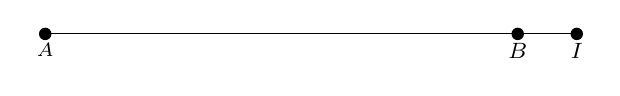
\begin{tikzpicture}[scale=1.5, font=\footnotesize, line join=round, line cap=round, >=stealth]
				\coordinate[label=below:\scriptsize$A$] (A) at (0,0);
				\coordinate[label=below:$B$] (B) at (4,0);
				\coordinate[label=below:$I$] (I) at (4.5,0);
				\draw (A)--(I);
				\foreach \diem in {A,B,I}	\fill (\diem)circle(1.5pt);
			\end{tikzpicture}
		\end{center}
		Ta có
		\begin{eqnarray*}
			&&MA=3MB\Leftrightarrow{\overrightarrow{MA}^2}=9\overrightarrow{MB}^2	\\
			&\Leftrightarrow&\left(\overrightarrow{MI}+\overrightarrow{IA}\right)^2=9\left(\overrightarrow{MI}+\overrightarrow{IB}\right)^2\\&\Leftrightarrow& IA^2-9IB^2+2\overrightarrow{MI}\left(\overrightarrow{IA}-9\overrightarrow{IB}\right)=8MI^2.\quad(1)
		\end{eqnarray*}  \\
		Gọi $I$ thỏa mãn $\overrightarrow{IA}-9\overrightarrow{IB}=\overrightarrow{0}\Leftrightarrow \overrightarrow{BI}=\dfrac{1}{8}\overrightarrow{AB}$ nên $IB=\dfrac{1}{2};IA=\dfrac{9}{2}$.\\
		Từ $(1)$ suy ra $8MI^2=18\Leftrightarrow MI=\dfrac{3}{2}$ suy ra $M\in S\left(I;\dfrac{3}{2}\right)$.}
\end{ex}

\begin{ex}%[2H5H3-3]
	Trong KG $Oxyz$, mặt cầu $(S)$ qua bốn điểm $A(3;3;0)$, $B(3;0;3)$, $C(0;3;3)$, $D(3;3;3)$. Phương trình mặt cầu $(S)$ là
	\choice
	{$\left(x-\dfrac{3}{2}\right)^2+\left(y-\dfrac{3}{2}\right)^2+\left(z-\dfrac{3}{2}\right)^2=\dfrac{3\sqrt{3}}{2}$}
	{$\left(x-\dfrac{3}{2}\right)^2+\left(y+\dfrac{3}{2}\right)^2+\left(z-\dfrac{3}{2}\right)^2=\dfrac{27}{4}$}
	{$\left(x-\dfrac{3}{2}\right)^2+\left(y-\dfrac{3}{2}\right)^2+\left(z+\dfrac{3}{2}\right)^2=\dfrac{27}{4}$}
	{\True $\left(x-\dfrac{3}{2}\right)^2+\left(y-\dfrac{3}{2}\right)^2+\left(z-\dfrac{3}{2}\right)^2=\dfrac{27}{4}$}
	\loigiai{
		Gọi phương trình mặt cầu $(S)\colon x^2+y^2+z^2-2ax-2by-2cz+d=0$ $(a^2+b^2+c^2-d>0)$.\\
		Vì mặt cầu đi qua $4$ điểm nên
		\begin{eqnarray*}
			&&\heva{&18-6a-6b+d=0 \\&18-6a-6c+d=0 \\&18-6b-6c+d=0 \\&27-6a-6b-6c+d=0}\\&\Leftrightarrow& \heva{&-6a-6b+d=-18 \\&-6a-6c+d=-18 \\&-6b-6c+d=-18 \\&-6a-6b-6c+d=-27}\\&\Leftrightarrow& \heva{&a=\dfrac{3}{2} \\&b=\dfrac{3}{2} \\&c=\dfrac{3}{2} \\&d=0.}	
		\end{eqnarray*}
		Suy ra tâm $I\left(\dfrac{3}{2};\dfrac{3}{2};\dfrac{3}{2}\right)$ bán kính $R=\sqrt{\left(\dfrac{3}{2}\right)^2+\left(\dfrac{3}{2}\right)^2+\left(\dfrac{3}{2}\right)^2}=\dfrac{3\sqrt{3}}{2}$.\\
		Vậy phương trình mặt cầu $\left(x-\dfrac{3}{2}\right)^2+\left(y-\dfrac{3}{2}\right)^2+\left(z-\dfrac{3}{2}\right)^2=\dfrac{27}{4}$.}
\end{ex}

\begin{ex}%[2H5H3-2]
	Trong KG $Oxyz$, cho tứ diện đều $ABCD$ có $A(0;1;2)$ và hình chiếu vuông góc của $A$ trên mặt phẳng $(BCD)$ là $H(4;-3;-2)$. Tìm tọa độ tâm $I$ của mặt cầu ngoại tiếp tứ diện $ABCD$.
	\choice
	{\True $I(3;-2;-1)$}
	{$I(2;-1;0)$}
	{$I(3;-2;1)$}
	{$I(-3;-2;1)$}
	\loigiai{
		Gọi $I(a;b;c)\Rightarrow \overrightarrow{IA}=(-a;1-b;2-c);\overrightarrow{IH}=(4-a;-3-b;-2-c)$.\\
		$ABCD$ là tứ diện đều nên tâm $I$ của mặt cầu ngoại tiếp trùng với trọng tâm tứ diện $\Rightarrow \overrightarrow{IA}=-3\overrightarrow{IH}$ $\Rightarrow \heva{&-a=-3(4-a) \\&1-b=-3(-3-b) \\&2-c=-3(-2-c)}\Rightarrow \heva{&a=3 \\&b=-2 \\&c=-1.}$\\ Vậy $I(3;-2;-1)$.}
\end{ex}

\begin{ex}%[2H5V3-3]
	Trong không gian tọa độ $Oxyz$, mặt cầu $(S)$ đi qua điểm $O$ và cắt các tia $Ox$, $Oy$, $Oz$ lần lượt tại các điểm $A$, $B$, $C$ khác $O$ thỏa mãn tam giác $ABC$ có trọng tâm là điểm $G(-6;-12;18)$. Tọa độ tâm của mặt cầu $(S)$ là
	\choice
	{$(9;18;-27)$}
	{$(-3;-6;9)$}
	{$(3;6;-9)$}
	{\True $(-9;-18;27)$}
	\loigiai{
		Gọi tọa độ các điểm trên ba tia $Ox$, $Oy$, $Oz$ lần lượt là $A(a;0;0)$, $B(0;b;0)$, $C(0;0;c)$ với $a$, $b$, $c>0$.\\
		Vì $G$ là trọng tâm tam giác $ABC$ nên $\heva{&\dfrac{a}{3}=-6 \\&\dfrac{b}{3}=-12 \\&\dfrac{c}{3}=18}\Leftrightarrow \heva{&a=-18 \\&b=-36 \\&c=54.}$\\
		Gọi phương trình mặt cầu $(S)$ cần tìm là $x^2+y^2+z^2-2mx-2ny-2pz+q=0$.\\
		Vì $(S)$ qua các điểm $O$, $A$, $B$, $C$ nên ta có hệ:
		$\heva{&q=0 \\&36m+q=-18^2 \\&72n+q=-36^2 \\&-108p+q=-54^2}\Leftrightarrow \heva{&m=-9 \\&n=-18 \\&p=27 \\&q=0.}$\\
		Vậy tọa độ tâm mặt cầu $(S)$ là $(-9;-18;27)$.}
\end{ex}

\begin{ex}%[2H5V3-3]
	Trong hệ trục tọa độ $Oxyz$, cho mặt cầu $$(S)\colon{(x-\cos \alpha)^2}+(y-\cos \beta)^2+(z-\cos \gamma)^2=4$$ với $\alpha$, $\beta$ và $\gamma$ lần lượt là ba góc tạo bởi tia $Ot$ bất kì với $3$ tia $Ox$, $Oy$ và $Oz$. Biết rằng mặt cầu $(S)$ luôn tiếp xúc với hai mặt cầu cố định. Tổng diện tích của hai mặt cầu cố định đó bằng
	\choice
	{\True $40\pi$}
	{$4\pi$}
	{$20\pi$}
	{$36\pi$}
	\loigiai{
		Ta dễ dàng chứng minh được: $\cos^2\alpha +\cos^2\beta +\cos^2\gamma =1$.\\
		Mặt cầu $(S)$ có tâm $I(\cos \alpha;\cos \beta;\cos \gamma)$.\\
		Suy ra tâm $I$ thuộc mặt cầu $(S')$ có tâm $O(0;0;0)$, $R=\sqrt{\cos^2\alpha +\cos^2\beta +\cos^2\gamma}=1$.\\
		Mặt cầu $(S)$ luôn tiếp xúc với hai mặt cầu $(S_1)$, $(S_2)$.\\
		Mặt cầu $(S_1)$ có tâm là $O$, bán kính $R_1=\left| OI-R\right|=\left| 1-2\right|=1$.\\
		Mặt cầu $(S_2)$ có tâm là $O$, bán kính $R_2=OI+R=1+2=3$.\\
		Vậy tổng diện tích hai mặt cầu bằng $4\pi (R_1^2+R_2^2)=4\pi (1^2+3^2)=40\pi$.}
\end{ex}

\begin{ex}%[2H5H3-3]
	Trong KG $Oxyz$, cho điểm $M(1;-2;3)$. Gọi $I$ là hình chiếu vuông góc của $M$ trên trục $Ox$. Phương trình nào dưới đây là phương trình mặt cầu tâm $I$ bán kính $IM$?
	\choice
	{\True $(x-1)^2+y^2+z^2=13$}
	{$(x+1)^2+y^2+z^2=17$}
	{$(x+1)^2+y^2+z^2=13$}
	{$(x-1)^2+y^2+z^2=\sqrt{13}$}
	\loigiai{
		Hình chiếu vuông góc của $M$ trên trục $Ox$ là $I(1;0;0)\Rightarrow IM=\sqrt{13}$.\\Suy ra phương trình mặt cầu tâm $I$ bán kính $IM$ là $(x-1)^2+y^2+z^2=13$.}
\end{ex}

\begin{ex}%[2H5H3-3]
	Trong KG $Oxyz$, cho điểm $I(1;-2;3)$. Viết phương trình mặt cầu tâm $I$, cắt trục $Ox$ tại hai điểm $A$ và $B$ sao cho $AB=2\sqrt{3}$
	\choice
	{\True $(x-1)^2+(y+2)^2+(z-3)^2=16$}
	{$(x-1)^2+(y+2)^2+(z-3)^2=20$}
	{$(x-1)^2+(y+2)^2+(z-3)^2=25$}
	{$(x-1)^2+(y+2)^2+(z-3)^2=9$}
	\loigiai{
		Gọi $H$ là trung điểm $AB$ suy ra $H$ là hình chiếu vuông góc của $I$ lên $Ox$ nên $H(1;0;0)$.\\
		$IH=\sqrt{13}\Rightarrow R=IA=\sqrt{IH^2+AH^2}=4$.\\
		Phương trình mặt cầu là $(x-1)^2+(y+2)^2+(z-3)^2=16$}
\end{ex}

\begin{ex}%[2H5H3-3]
	Trong KG $Oxyz$, cho điểm $M(1;-2;3)$. Gọi $I$ là hình chiếu vuông góc của $M$ trên trục $Ox$. Phương trình nào sau đây là phương trình mặt cầu tâm $I$ bán kính $IM$?
	\choice
	{$(x-1)^2+y^2+z^2=\sqrt{13}$}
	{\True $(x-1)^2+y^2+z^2=13$}
	{$(x+1)^2+y^2+z^2=13$}
	{$(x+1)^2+y^2+z^2=17$}
	\loigiai{
		Với điểm $M(1;-2;3)$ thì hình chiếu vuông góc của $M$ trên trục $Ox$ là $I(1;0;0)$ suy ra $IM=\sqrt{13}$.\\ Vậy phương trình mặt cầu tâm $I(1;0;0)$ bán kính $IM$ là $(x-1)^2+y^2+z^2=13$.}
\end{ex}

\begin{ex}%[2H5H3-3]
	Trong KG $Oxyz$, cho tứ diện $ABCD$ có tọa độ đỉnh $A(2; 0; 0)$, $B(0;4; 0)$, $C(0; 0;6)$, $A(2;4;6)$. Gọi $(S)$ là mặt cầu ngoại tiếp tứ diện $ABCD$. Viết phương trình mặt cầu $(S')$ có tâm trùng với tâm của mặt cầu $(S)$ và có bán kính gấp $2$ lần bán kính của mặt cầu $(S)$.
	\choice
	{\True $(x-1)^2+(y-2)^2+(z-3)^2=56$}
	{$x^2+y^2+z^2-2x-4y-6z=0$}
	{$(x+1)^2+(y+2)^2+(z+3)^2=14$}
	{$x^2+y^2+z^2-2x+4y+6z-12=0$}
	\loigiai{
		Gọi phương trình mặt cầu $(S)$ có dạng $x^2+y^2+z^2-2ax-2by-2cz+d=0$.\\
		Vì $(S)$ là mặt cầu ngoại tiếp tứ diện $ABCD$ nên ta có
		\begin{eqnarray*}
			&&\heva{&2^2+0^2+0^2-2\cdot a\cdot 2-2\cdot b\cdot 0-2\cdot c\cdot 0+d=0 \\&0^2+4^2+0^2-2\cdot a\cdot 0-2\cdot b\cdot 4-2\cdot c\cdot 0+d=0 \\&0^2+0^2+6^2-2\cdot a\cdot 0-2\cdot b\cdot 0-2\cdot c\cdot 6+d=0 \\&2^2+4^2+6^2-2\cdot a\cdot 2-2\cdot b\cdot 4-2\cdot c\cdot 6+d=0}\\&\Leftrightarrow&\heva{&-4a+d=-4 \\&-8b+d=-16 \\&-12c+d=-36 \\&-4a-8b-12c+d=-56}\\&\Leftrightarrow&\heva{&a=1 \\&b=2 \\&c=3 \\&d=0.}
		\end{eqnarray*}
		Suy ra $x^2+y^2+z^2-2x-4y-6z=0\Rightarrow I(1; 2; 3)$ và $R=\sqrt{14} \Rightarrow R'=2\sqrt{14}$.\\
		Vậy mặt cầu $(S')$ có tâm $I(1; 2; 3)$ và $R'=2\sqrt{14}$ có phương trình $$(x-1)^2+(y-2)^2+(z-3)^2=56.$$}
\end{ex}

\begin{ex}%[2H5H3-3]
	Trong KG $Oxyz$, mặt cầu tâm $I(2;1;-3)$ và tiếp xúc với trục $Oy$ có phương trình là
	\choice
	{$(x-2)^2+(y-1)^2+(z+3)^2=4$}
	{\True $(x-2)^2+(y-1)^2+(z+3)^2=13$}
	{$(x-2)^2+(y-1)^2+(z+3)^2=9$}
	{$(x-2)^2+(y-1)^2+(z+3)^2=10$}
	\loigiai{
		Gọi $M$ là hình chiếu của $I$ trên $Oy$ $\Rightarrow M(0;1;0)$
		Mặt cầu $(S)$ tâm $I(2;1;-3)$ và tiếp xúc với trục $Oy$ có bán kính $IM=\sqrt{13}$.\\
		Vậy $(S)$ có phương trình $(x-2)^2+(y-1)^2+(z+3)^2=13$.}
\end{ex}

\begin{ex}%[2H5H3-3]
	Trong KG $Oxyz$, cho mặt cầu $(S)\colon{(x-1)^2}+(y-1)^2+z^2=4$. Một mặt cầu $(S')$ có tâm $I'(9;1;6)$ và tiếp xúc ngoài với mặt cầu $(S)$. Phương trình mặt cầu $(S')$ là
	\choice
	{\True $(x-9)^2+(y-1)^2+(z-6)^2=64$}
	{$(x-9)^2+(y-1)^2+(z-6)^2=144$}
	{$(x-9)^2+(y-1)^2+(z-6)^2=36$}
	{$(x+9)^2+(y+1)^2+(z+6)^2=25$}
	\loigiai{
		Gọi $I(1;1;0)$, $R=2$. $II'=10$.\\
		Gọi $R'$ là bán kính của mặt cầu $(S')$.\\
		Theo giả thiết, ta có $R'+R=II'\Leftrightarrow R'=II'-R=8$.\\
		Khi đó phương trình mặt cầu $(S')\colon (x-9)^2+(y-1)^2+(z-6)^2=64$.}
\end{ex}

\begin{ex}%[2H5V3-3]
	Trong KG $Oxyz$, cho điểm $H(1;2;-2)$. Mặt phẳng $(\alpha)$ đi qua $H$ và cắt các trục $Ox$, $Oy$, $Oz$ tại $A$, $B$, $C$ sao cho $H$ là trực tâm tam giác $ABC$. Viết phương trình mặt cầu tâm $O$ và tiếp xúc với mặt phẳng $(\alpha)$.
	\choice
	{$x^2+y^2+z^2=81$}
	{$x^2+y^2+z^2=1$}
	{\True $x^2+y^2+z^2=9$}
	{$x^2+y^2+z^2=25$}
	\loigiai{
		Ta có $H$ là trực tâm tam giác $ABC$ $\Rightarrow OH\perp (ABC)$.\\
		Thật vậy
		$\heva{&OC\perp OA \\&OC\perp OB}\Rightarrow OC\perp AB$.  (1)\\
		Mà $CH\perp AB$ (vì $H$ là trực tâm tam giác $ABC$). (2)\\
		Từ (1) và (2) suy ra $AB\perp (OHC)$ $\Rightarrow AB\perp OH$.  (*)\\
		Tương tự $BC\perp (OAH)\Rightarrow BC\perp OH$. (**)\\
		Từ (*) và (**) suy ra $OH\perp (ABC)$.\\
		Khi đó mặt cầu tâm $O$ tiếp xúc mặt phẳng $(ABC)$ có bán kính $R=OH=3$.\\
		Vậy mặt cầu tâm $O$ và tiếp xúc với mặt phẳng $(\alpha)$ là $(S)\colon x^2+y^2+z^2=9$.}
\end{ex}

\Closesolutionfile{ans}
% \indapan{10}{ans/ans-2-C5-B3-CD1-D2-LC}
%PHẦN III. Câu trắc nghiệm đúng sai. Trong mỗi ý A), B), C), D) ở mỗi câu, thí sinh chọn đúng hoặc sai.
\TNTF
\Opensolutionfile{ans}[ans/ans-C5B3CD1_22-30-DS]
%Câu55
\begin{ex}%[2H5N3-3]
	Trong KG $Oxyz$, cho mặt cầu $(S)$ có tâm $I(0;-2;1)$, bán kính bằng $ 2 $. Các mệnh đề sau đây đúng hay sai?
	\choiceTF
	{Phương trình của mặt cầu $(S)$ là $x^2+(y+2)^2+(z-1)^2=2$}
	{Phương trình của mặt cầu $(S)$ là $x^2+(y-2)^2+(z+1)^2=2$}
	{Phương trình của mặt cầu $(S)$ là $x^2+(y-2)^2+(z+1)^2=4$}
	{\True Phương trình của mặt cầu $(S)$ là $x^2+(y+2)^2+(z-1)^2=4$}
	\loigiai{
		Vì phương trình mặt cầu tâm $I(a ; b ; c)$ và bán kính bằng $R$ là $$(x-a)^2+(y-b)^2+(z-c)^2=R^2.$$
		Vậy phương trình mặt cầu $(S)$ có tâm $I(0 ;-2 ; 1)$ và bán kính bằng $ 2 $ là $$x^2+(y+2)^2+(z-1)^2=4.$$
		\begin{itemchoice}
			\itemch Sai.
			\itemch Sai.
			\itemch Sai.
			\itemch Đúng.	
		\end{itemchoice}
	}
\end{ex}
%câu 56
\begin{ex}%[2H5H3-3]
	Trong KG $Oxyz$, cho hai điểm $I(1;1;1)$ và $A(1;2;3)$. Gọi $(S)$ là mặt cầu tâm $ I $ và đi qua điểm $ A $. Các mệnh đề sau đây đúng hay sai?
	\choiceTF[t]
	{Phương trình mặt cầu $ (S)$ là $(x+1)^{2}+(y+1)^{2}+(z+1)^{2}=5$}
	{Phương trình mặt cầu $ (S)$ là $(x+1)^{2}+(y+1)^{2}+(z+1)^{2}=29$}
	{\True Phương trình mặt cầu $ (S)$ là $(x-1)^{2}+(y-1)^{2}+(z-1)^{2}=5$}
	{Phương trình mặt cầu $ (S) $ là $(x-1)^2+(y-1)^2+(z-1)^2=25$}
	\loigiai{Vì $R=I A=\sqrt{(1-1)^2+(2-1)^2+(3-1)^2}=\sqrt5$.\\
		Vậy phương trình mặt cầu tâm $I$ và đi qua điểm $A$ có phương trình là
		
		$\left(x-x_{I}\right)^2+\left(y-y_{I}\right)^2+\left(z-z_{I}\right)^2=R^2 \Rightarrow(x-1)^2+(y-1)^2+(z-1)^2=5$.
		\begin{itemchoice}
			\itemch Sai. 
			\itemch Sai.
			\itemch Đúng.
			\itemch Sai.
	\end{itemchoice}}
\end{ex}
%Câu 57
\begin{ex}%[2H5H3-3]
	Trong KG $Oxyz$, cho hai điểm $A(2;-1;-3)$; $B(0;3;-1)$. Gọi $ (S) $ là mặt cầu đường kính $ AB $. Các mệnh đề sau đây đúng hay sai?
	\choiceTF[t]
	{\True Phương trình của mặt cầu $ (S) $ là $(x-1)^2+(y-1)^2+(z+2)^2=6$}
	{Phương trình của mặt cầu $ (S) $ là $(x-1)^2+(y-1)^2+(z+2)^2=24$}
	{Phương trình của mặt cầu $ (S) $ là $(x+1)^2+(y+1)^2+(z-2)^2=24$}
	{\True Phương trình của mặt cầu có tâm là trung điểm $AB$ và đi qua hai điểm $A$, $B$ là $(x-1)^2+(y-1)^2+(z+2)^2=6$}
	\loigiai{
		Vì tâm $I$ của mặt cầu $ (S) $ là trung điểm của $A B$ suy ra	$I(1 ; 1 ;-2)$ và bán kính $R=\dfrac{1}{2}AB=\dfrac{1}{2} \sqrt{4+16+4}=\dfrac{1}{2} \sqrt{24}$.\\
		Vậy phương trình của mặt cầu đường kính $ AB $ là	
		$$(x-1)^2+(y-1)^2+(z+2)^2=6.$$
		\begin{itemchoice}
			\itemch Đúng.
			\itemch Sai.
			\itemch Sai.
			\itemch Đúng. Vì mặt cầu có tâm là trung điểm $AB$ và đi qua hai điểm $A$, $B$ là mặt cầu đường kính $ AB $.
	\end{itemchoice}}
\end{ex}
%Câu 58
\begin{ex}%[2H5H3-2]
	Gọi $(S)$ là mặt cầu đi qua bốn điểm $A(2;0;0)$, $B(1;3;0)$, $C(-1;0;3)$, $D(1;2;3)$. Các mệnh đề sau đây đúng hay sai?
	\choiceTF[t]
	{Mặt cầu $(S)$ có tọa độ tâm là $(1;-1;1)$}
	{\True Mặt cầu $(S)$ có tọa độ tâm là $(0;1;1)$}
	{Bán kính $R$ của mặt cầu $(S)$ là $R=6$}
	{\True Bán kính $R$ của mặt cầu $(S)$ là $R=\sqrt{6}$}
	\loigiai{
		Vì giả sử $I(a;b;c)$ là tâm mặt cầu đi qua bốn điểm $A$, $B$, $C$, $D$. Khi đó\\
		\begin{eqnarray*}
			& 				 & \heva{&AI^2 = BI^2\\&AI^2=CI^2\\&AI^2=DI^2} \\
			&\Leftrightarrow & \heva{&(a-2)^2+b^2+c^2=(a-1)^2+(b-3)^2+c^2\\&(a-2)^2+b^2+c^2=(a+1)^2+b^2+(c-3)^2\\&(a-2)^2+b^2+c^2=(a-1)^2+(b-2)^2+(c-3)^2} \\
			& \Leftrightarrow & \heva{&a-3b=-3\\&a-c=-1\\& a-2b-3c=-5} \\
			& \Leftrightarrow & \heva{&a=0\\&b=1\\&c=1.}
		\end{eqnarray*}
		Vậy $I(0; 1; 1)$; bán kính $R=I A=\sqrt{2^2+1^2+1^2}=\sqrt6$.
		\begin{itemchoice}
			\itemch Sai. 
			\itemch Đúng.
			\itemch Sai.
			\itemch Đúng.
	\end{itemchoice}} 
\end{ex}
%Câu 59
\begin{ex}%[2H5V3-2]
	Trong không gian với hệ trục tọa độ $Oxyz$, cho mặt cầu $(S)$ có tâm nằm trên mặt phẳng $(O x y)$ và đi qua ba điểm $A(1;2;-4)$, $B(1;-3;1)$, $C(2;2;3)$. Các mệnh đề sau đây đúng hay sai?
	\choiceTF[t]
	{Tọa độ tâm $(I)$ của mặt cầu $(S)$ là $(2;-1;0)$}
	{\True Tọa độ tâm $(I)$ của mặt cầu $(S)$ là $(-2;1;0)$}
	{\True Bán kính $R$ của mặt cầu $(S)$ là $R=\sqrt{26}$}
	{Bán kính $R$ của mặt cầu $(S)$ là $R=26$}
	\loigiai{
		Vì giả sử tâm $I(a;b;c)$ và phương trình mặt cầu $(S)$ là $$x^2+y^2+z^2-2ax-2by-2cz+d=0.$$
		Do $I \in (Oxy) \Leftrightarrow c=0 \Leftrightarrow(S)\colon x^2+y^2+z^2-2ax-2by+d=0$.\\
		Ta có $\heva{&A\in (S)\\&B\in (S)\\& C \in (S)} \Leftrightarrow \heva{&2a+4b-d=21 \\&2a-6b-d=11 \\& 4a+4b-d=17}\Leftrightarrow\heva{&a=-2 \\& b=1 \\ &d=-21.}$\\
		Vậy $I(-2;1;0)$ và $R=\sqrt{26}$.
		\begin{itemchoice}
			\itemch	Sai.
			\itemch	Đúng.
			\itemch	Đúng.
			\itemch	Sai.
	\end{itemchoice}}
\end{ex}
%Câu 60
\begin{ex}%[2H5H3-3]
	Trong không gian với hệ trục tọa độ $Oxyz$, cho điểm $A(1;1;2)$, $B(3;2;-3)$. Mặt cầu $(S)$ có tâm $I$ thuộc $Ox$ và đi qua hai điểm $A$, $B$. Các mệnh đề sau đây đúng hay sai?
	\choiceTF[t]
	{\True Tọa độ tâm $(I)$ của mặt cầu $(S)$ là $I(4;0;0)$}
	{Bán kính $R$ của mặt cầu $(S)$ là $R=14$}
	{\True Mặt cầu $(S)$ có phương trình $x^2+y^2+z^2-8x+2=0$}
	{Mặt cầu $(S)$ có phương trình $x^2+y^2+z^2-8x-2=0$}
	\loigiai{
		Vì giả sử $I(a;0;0) \in Ox \Rightarrow \overrightarrow{IA}(1-a;1;2)$; $ \overrightarrow{IB}(3-a;2;-3)$.\\
		Do $(S)$ đi qua hai điểm $A$, $B$ nên
		\begin{eqnarray*}
			& & IA=IB \\
			& \Leftrightarrow &  \sqrt{(1-a)^2+5}=\sqrt{(3-a)^2+13} \\
			& \Leftrightarrow & 4 a=16 \\
			& \Leftrightarrow & a=4.
		\end{eqnarray*} 
		Suy ra mặt cầu $(S)$ có tâm $I(4;0;0)$, bán kính $R=IA=\sqrt{14}$.\\
		Vậy	$(S)$ là $(x-4)^2+y^2+z^2=14 \Leftrightarrow x^2+y^2+z^2-8x+2=0$.
		\begin{itemchoice}
			\itemch Đúng. 
			\itemch Sai.
			\itemch Đúng.
			\itemch Sai.
		\end{itemchoice}
	}
\end{ex}
%Câu 61
\begin{ex}%[2H5V3-3]
	Trong KG $Oxyz$, mặt cầu $(S)$ đi qua điểm $A(1;-1;4)$ và tiếp xúc với các mặt phẳng tọa độ. Các mệnh đề sau đây đúng hay sai?
	\choiceTF[t]
	{Mặt cầu $(S)$ có phương trình $(x-3)^2+(y+3)^2+(z+3)^2=16$}
	{\True Mặt cầu $(S)$ có phương trình $(x-3)^2+(y+3)^2+(z-3)^2=9$}
	{Mặt cầu $(S)$ có phương trình $(x+3)^2+(y-3)^2+(z+3)^2=36$}
	{Mặt cầu $(S)$ có phương trình $(x+3)^2+(y-3)^2+(z-3)^2=49$}
	\loigiai{
		Vì giả sử $I(a;b;c)$ là tâm của mặt cầu $(S)$. Mặt cầu $(S)$ tiếp xúc với các mặt phẳng tọa độ $\mathrm{d}\Big(I,(Oxy)\Big)=\mathrm{d}\Big(I,(Oyz)\Big)=\mathrm{d}\Big(I,(Oxz)\Big) \Leftrightarrow|a|=|b|=|c|=R$.\\
		Mặt cầu $(S)$ đi qua $A(1;-1;4)$. Ta có
		\begin{eqnarray*}
			& \Rightarrow & \heva{& IA=R \\& a>0;c>0;b<0}\\
			& \Leftrightarrow & \heva{& IA^2=R^2\\& a>0; c>0; b < 0} \\
			& \Leftrightarrow & \heva{& (a-1)^2+(b+1)^2+(c-4)^2=R^2\\& a=c=-b=R>0} \\
			& \Leftrightarrow & \heva{& (a-1)^2+(-a+1)^2+(a-4)^2=a^2\\& a=c=-b=R>0 } \\
			& \Leftrightarrow & \heva{& 2a^2-12a+18=0 \\& a=c=-b=R>0} \\
			& \Leftrightarrow & \heva{& a=c=3\\& b=-3 \\& R=3.}
		\end{eqnarray*}
		Vậy $(S)\colon (x-3)^2+(y+3)^2+(z-3)^2=9$.
		\begin{itemchoice}
			\itemch Sai.
			\itemch Đúng.
			\itemch Sai.
			\itemch Sai.
	\end{itemchoice}}
\end{ex}
\Closesolutionfile{ans}
% \indapan{3}{ans/ans-C5B3CD1_22-30-DS}

%PHẦN III. Câu trắc nghiệm trả lời ngắn. Mỗi câu hỏi thí sinh chỉ trả lời đáp án.
\TNSA
\Opensolutionfile{ans}[ans/ans-C5B3CD1_22-30-KQ]
%CÂU 62
\begin{ex}%[2H5N3-3]
	Trong KG $Oxyz$, mặt cầu $(S)$ có tâm $I(0; 1;-2)$ và bán kính bằng $ 3 $. Phương trình của $(S)$ có dạng $ x^2+y^2+z^2-2ax-2by-2cz+d=0 $. Tìm $ d $.
	\shortans{$ -4 $}
	\loigiai{
		Phương trình mặt cầu tâm $I(a; b; c)$ và bán kính bằng $R$ là $(x-a)^2+(y-b)^2+(z-c)^2=R^2$.\\
		Ta có mặt cầu tâm $I(0;1;-2)$, bán kính bằng $ 3 $ có phương trình là $$x^2+(y-1)^2+(z+2)^2=9\Leftrightarrow x^2+y^2+z^2-2y+4z-4=0.$$}
\end{ex}
%Câu 63
\begin{ex}%[2H5N3-2]
	Trong KG $Oxyz$, cho mặt cầu có tâm $I(1;-4;3)$ và đi qua điểm $A(5;-3;2)$. Tính bán kính của mặt cầu đã cho (làm tròn kết quả đến hàng phần nghìn).
	\shortans{$ 4{,}24 $}
	\loigiai{Mặt cầu tâm $I(1;-4;3)$ và đi qua điểm $A(5;-3;2)$ nên bán kính $R=IA=3\sqrt{2}\approx 4{,}24$.}
\end{ex}
%Câu 64
\begin{ex}%[2H5H3-3]
	Trong KG $Oxyz$, cho hai điểm $A(1;1;1)$ và $B(1;-1;3)$. Phương trình mặt cầu có đường kính $AB$ có dạng $ x^2+y^2+z^2-2ax-2by-2cz+d=0$. Tính tổng $S= a+b+c+d$.
	\shortans{$ 6 $}
	\loigiai{Gọi $I$ là tâm của mặt cầu đường kính $AB$.\\
		Khi đó $ I $ là trung điểm của đoạn $ AB \Rightarrow I(1;0;2)$.\\
		Bán kính của mặt cầu là $R=\dfrac{1}{2}AB=\dfrac{1}{2}\sqrt{(1-1)^2+(-1-1)^2+(3-1)^2}=\sqrt2$.\\	
		Suy ra phương trình mặt cầu là $(x-1)^2+y^2+(z-2)^2=2 \Leftrightarrow x^2+y^2+z^2-2x-4z+3=0$.\\
		Vậy $S= a+b+c+d=1+2+3=6 $.}
\end{ex}
%Câu 65
\begin{ex}%[2H5H3-2]
	Trong KG $Oxyz$, cho $A(-1; 0; 0)$, $B(0; 0; 2)$, $C(0;-3; 0)$. Tính bán kính mặt cầu ngoại tiếp tứ diện $OABC$ (làm tròn đến hàng phần nghìn).
	\shortans{$ 1{,}87 $}
	\loigiai{Gọi $(S)$ là mặt cầu ngoại tiếp tứ diện $OABC$.\\	
		Phương trình mặt cầu $(S)$ có dạng $x^2+y^2+z^2-2ax-2by-2cz+d=0$.\\	
		Vì $O$, $ A$, $B$, $C$ thuộc $(S)$ nên ta có
		$ \heva{& d=0 \\& 1+2a+d = 0\\& 4-4c+d=0\\& 9+6b+d=0}\Leftrightarrow \heva{& a=-\dfrac{1}{2}\\ & b=-\dfrac{3}{2}\\& c=1 \\& d=0.} $\\
		Vậy bán kính mặt cầu $(S)$ là $R=\sqrt{a^2+b^2+c^2-d}=\sqrt{\dfrac{1}{4}+\dfrac{9}{4}+1}=\dfrac{\sqrt{14}}{2}\approx 1{,}87$.
	}
\end{ex}
%Câu 66
\begin{ex}%[2H5V3-2]
	Trong KG $Oxyz$, gọi $I(a;b;c)$ là tâm mặt cầu đi qua điểm $A(1;-1;4)$ và tiếp xúc với tất cả các mặt phẳng tọa độ. Tính $P=a-b+c$.
	\shortans{$ 9 $}
	\loigiai{Vì mặt cầu tâm $I$ tiếp xúc với các mặt phẳng tọa độ nên\\
		$\mathrm{d}\Big(I,(Oxy)\Big)=\mathrm{d}\Big(I,(Oyz)\Big)=\mathrm{d}\Big(I,(Oxz)\Big) \Leftrightarrow |a|=|b|=|c| \Leftrightarrow\hoac{&  a=b=c \\& a=b=-c \\& a=-b=c \\& a=-b=-c.}$\\	
		Nhận thấy chỉ có trường hợp $a=-b=c$ thì phương trình $AI=\mathrm{d}\Big(I,(Oxy)\Big)$ có nghiệm, các trường hợp còn lại vô nghiệm.\\	
		Thật vậy, với $a=-b=c$ thì $I(a;-a; a)$.\\
		$AI=\mathrm{d}\Big(I,(Oxy)\Big) \Leftrightarrow \left(a-1\right)^2+\left(a-1\right)^2+\left(a-4\right)^2=a^2 \Leftrightarrow a^2-6a+9=0 \Leftrightarrow a=3$.\\
		Khi đó $P=a-b+c=9$.
	}
\end{ex}
%Câu 67
\begin{ex}%[2H5V3-2]
	Trong không gian $O x y z$, tìm giá trị dương của $m$ (làm tròn đến hàng phần nghìn) sao cho mặt phẳng $(Oxy)$ tiếp xúc với mặt cầu $\left(x-3\right)^2+y^2\left(z-2\right)^2=m^2+1$.
	\shortans{$ 1{,}73 $}
	\loigiai{Mặt cầu $(S)\colon \left(x-3\right)^2+y^2\left(z-2\right)^2=m^2+1$ có tâm $I(3;0;2)$, bán kính $R=\sqrt{m^2+1}$.\\	
		$(S)$ tiếp xúc với $(Oxy) \Leftrightarrow \mathrm{d}\left(I,(Oxy)\right)=R \Leftrightarrow 2=\sqrt{m^2+1} \Leftrightarrow m^2=3 \Leftrightarrow m=\sqrt3 \approx 1{,}73$ (do $m>0$).}
	
\end{ex}
%Câu 68
\begin{ex}%[2H5V3-2]
	Trong không gian với hệ trục tọa độ $O x y z$, cho ba điểm $A(1 ; 2 ;-4), B(1 ;-3 ; 1), C(2 ; 2 ; 3)$. Tính đường kính của mặt cầu $(S)$ đi qua ba điểm trên và có tâm nằm trên mặt phẳng $(O x y)$ (Làm tròn kết quả đến hàng phần chục).
	\shortans{$ 10{,}2 $}
	\loigiai{
		Gọi tâm mặt cầu là $I(x;y;0)$. Ta có
		\begin{eqnarray*}
			& 				  & \heva{&IA=IB \\ &IA=IC} \\
			& \Leftrightarrow & \heva{&\sqrt{(x-1)^2+(y-2)^2+4^2}=\sqrt{(x-1)^2+(y+3)^2+1^2}\\&	\sqrt{(x-1)^2+(y-2)^2+4^2}=\sqrt{(x-2)^2+(y-2)^2+3^2}}\\
			& \Leftrightarrow & \heva{&(y-2)^2+4^2=(y+3)^2+1^2 \\&	x^2-2 x+1+16=x^2-4x+4+9}\\
			& \Leftrightarrow & \heva{&10y=10 \\& 2x=-4} \Leftrightarrow \heva{&x=-2\\&y=1.}
		\end{eqnarray*}
		$\Rightarrow l=2R=2\sqrt{(-3)^2+(-1)^2+4^2}=2\sqrt{26}\approx 10{,}2$.
	}
\end{ex}
%Câu 69
\begin{ex}%[2H5V3-2]
	Trong không gian $O x y z$, gọi $(S)$ là mặt cầu đi qua điểm $D(0 ; 1 ; 2)$ và tiếp xúc với các trục $O x, O y, O z$ tại các điểm $A(a ; 0 ; 0)$, $B(0 ; b ; 0)$, $C(0 ; 0 ; c)$ trong đó $a, b, c \in \mathbb{R} \backslash\{0 ; 1\}$. Tính bán kính của $(S)$ (làm tròn kết quả đến hàng phần chục).
	\shortans{$7{,}1$}
	\loigiai{
		Gọi $I$ là tâm của mặt cầu $(S)$.\\
		Vì $(S)$ tiếp xúc với các trục $O x, O y, O z$ tại các điểm $A(a ; 0 ; 0)$, $B(0 ; b ; 0)$, $C(0 ; 0 ; c)$ nên ta có $I A \perp Ox, I B \perp Oy, I C \perp Oz$ hay $A, B, C$ tương ứng là hình chiếu của $I$ trên $Ox, Oy, Oz \Rightarrow I(a;b;c)$.\\
		$\Rightarrow$ Mặt cầu $(S)$ có phương trình $x^2+y^2+z^2-2 ax-2 by-2cz+d=0$ với $a^2+b^2+c^2-d>0$.\\
		Vì $(S)$ đi qua $A$, $B$, $C$, $D$ nên ta có $ \heva{&a^2=b^2=c^2=d\\&5-2b-4c+d=0.} $\\
		Vì $a, b, c \in \mathbb{R} \backslash\{0 ; 1\}$ nên $0<d \neq 1$.\\
		Mặt khác, từ $(1) \Rightarrow R=\sqrt{a^2+b^2+c^2-d}=\sqrt{2d}$.
		\begin{itemize}
			\item TH1. Từ $(1) \Rightarrow b=c=\sqrt d$. Thay vào $(*)$ ta có $ 5-6 \sqrt d +d=0 \Leftrightarrow d=25$ (nhận).
			$\Rightarrow R=\sqrt{2.25}=5 \sqrt{2}$.
			\item TH2. Từ $(1) \Rightarrow b=c=-\sqrt d$. Thay vào $(*)$ ta có $ 5+6 \sqrt d+d=0$ (vô nghiệm).
			\item TH3. Từ $(1) \Rightarrow b=\sqrt{d}, c=-\sqrt d$. Thay vào $(*)$ ta có $ 5+2 \sqrt d +d=0$ (vô nghiệm).
			\item TH4. Từ $(1) \Rightarrow b=-\sqrt{d}, c=\sqrt d $. Thay vào $(*)$ ta có $ 5-2 \sqrt d +d=0$ (vô nghiệm).
		\end{itemize}
		Vậy mặt cầu $(S)$ có bán kính $R=5 \sqrt{2} \approx 7{,}1$.
	}
\end{ex}
%Câu 70
\begin{ex}%[2H5V3-3]
	Trong không gian với hệ trục tọa độ $Oxyz$, cho ba điểm $A(1; 0; 0), C(0; 0; 3), B(0; 2; 0)$. Tập hợp các điểm $M$ thỏa mãn $MA^2=MB^2+MC^2$ là mặt cầu có bán kính là bao nhiêu? (làm tròn kết quả đến hàng phần nghìn).
	\shortans{$ 1{,}41 $}
	\loigiai{
		Giả sử $M(x;y;z)$.\\
		Ta có $MA^2=(x-1)^2+y^2+z^2$; $MB^2=x^2+(y-2)^2+z^2$; $MC^2=x^2+y^2+(z-3)^2$.
		\begin{eqnarray*}
			& & MA^2 = MB^2 + MC^2\\
			& \Leftrightarrow & (x-1)^2+y^2+z^2=x^2+(y-2)^2+z^2+x^2+y^2+(z-3)^2\\
			& \Leftrightarrow & -2x+1=(y-2)^2+x^2+(z-3)^2 \\
			& \Leftrightarrow & (x+1)^2+(y-2)^2+(z-3)^2=2.
		\end{eqnarray*}
		Vậy tập hợp các điểm $M$ thỏa mãn $MA^2=MB^2+MC^2$ là mặt cầu có bán kính là $R=\sqrt 2 \approx 1{,}41$.
	}
\end{ex}
%Câu 71
\begin{ex}%[2H5H3-2]
	Trong không gian với hệ trục tọa độ $Oxyz$, xét mặt cầu $(S)$ có phương trình dạng $x^2+y^2+z^2-4x+2y-2az+10a=0$. Có tất cả bao nhiêu giá trị thực của $a$ để $(S)$ có chu vi đường tròn lớn bằng $8 \pi$.
	\shortans{$ 2 $}
	\loigiai{
		Đường tròn lớn có chu vi bằng $8 \pi$ nên bán kính của $(S)$ là $\dfrac{8\pi}{2 \pi}=4$.\\
		Từ phương trình của $(S)$ suy ra bán kính của $(S)$ là $\sqrt{2^2+1^2+a^2-10 a}$.\\
		Do đó $\sqrt{2^2+1^2+a^2-10a}=4 \Leftrightarrow \hoac{&a=-1\\&a=11.}$
	}
\end{ex}
%Câu 72
\begin{ex}%[2H5C3-2]
	Trong KG $Oxyz$, cho mặt cầu $(S)\colon (x-1)^2+(y-2)^2+(z-3)^2=25$ và hình nón $(H)$ có đỉnh $A(3; 2;-2)$ và nhận $AI$ làm trục đối xứng với $I$ là tâm mặt cầu. Một đường sinh của hình nón $(H)$ cắt mặt cầu tại $M, N$ sao cho $AM=3AN$. Tìm bán kính của mặt cầu đồng tâm với mặt cầu $(S)$ và tiếp xúc với các đường sinh của hình nón $(H)$ (làm tròn kết quả đến hàng phần nghìn).
	\shortans{$ 4{,}86 $}
	\loigiai{
		\begin{center}
			\begin{tikzpicture}[>=stealth,line join=round,line cap=round,font=\footnotesize,scale=.61]
				\path
				(0,0) coordinate (I)
				($(I)+(0,5)$) coordinate (A)
				($(I)-(1.2,0)$) coordinate (x)
				($(I)+(1.2,0)$) coordinate (y)
				(-.6,-.4) coordinate (z)
				(-.3,2.3) coordinate (N)
				(-.7,-1.3) coordinate (M)
				(-.45,.95) coordinate (K)
				%($(N)!.5!(M)$) coordinate (H)
				%($(N)!.7!(M)$) coordinate (A)
				;
				\draw (I) circle (4cm);
				\draw[dashed] (I) ellipse (1.2 and 0.5);
				\draw (4,0) arc (0:-180:4 and 1);
				\draw[dashed] (4,0) arc (0:180:4 and 1);
				\draw[dashed] (x)--(-.5,2.9) (y)--(.5,2.9) (N)--(M) (z)--(I)--(A) (I)--(K);
				\draw (N)--(A) (A)--(-.5,2.9) (A)--(.5,2.9);
				\foreach \p/\g in {I/0, N/135, M/-75, A/135, K/-130}
				\draw[fill=black] (\p) circle (1pt) node[shift=(\g:3mm)] {$\p$};
				
			\end{tikzpicture}
		\end{center}
		Gọi hình chiếu vuông góc của $I$ trên $M N$ là $K$.\\
		Dễ thấy $AN=NK=\dfrac{1}{3} AM$, mặt cầu $(S)$ có tâm $I(1; 2; 3)$ và bán kính $R=5$.\\	
		Ta có $AM \cdot AN=AI^2-R^2=4 \Rightarrow AN^2=\dfrac{4}{3} \Rightarrow KN=AN=\dfrac{2 \sqrt{3}}{3}$\\
		$\Rightarrow IK=\sqrt{IN^2-KN^2}=\dfrac{\sqrt{213}}{3}$.\\	
		Nhận thấy mặt cầu đồng tâm với mặt cầu $(S)$ và tiếp xúc với các đường sinh của hình nón $(H)$ chính là mặt cầu tâm $I(1; 2; 3)$ có bán kính $IK=\dfrac{\sqrt{213}}{3} \approx 4{,}86$.\\
	}
\end{ex}
%Câu 73
\begin{ex}%[2H5C3-2]
	Trong KG $Oxyz$, cho bốn điểm $A(0;-1;2)$, $B(2;-3; 0)$, $C(-2; 1; 1)$, $D(0;-1;3)$. Gọi $(L)$ là tập hợp tất cả các điểm $M$ trong không gian thỏa mãn đẳng thức $\overrightarrow{MA} \cdot \overrightarrow{MB}=\overrightarrow{MC} \cdot \overrightarrow{MD}=1$. Biết rằng $(L)$ là một đường tròn, đường tròn đó có bán kính $r$ bằng bao nhiêu? (Làm tròn kết quả đến hàng phần nghìn).
	\shortans{$ 1{,}66 $}
	\loigiai{
		Gọi $M(x; y; z)$ là tập hợp các điểm thỏa mãn yêu cầu bài toán. Ta có\\
		$\overrightarrow{AM}=(x; y+1; z-2)$, $\overrightarrow{BM}=(x-2; y+3; z)$, $ \overrightarrow{CM}=(x+2; y-1; z-1)$, $\overrightarrow{DM}=(x; y+1; z-3)$.\\
		Từ giả thiết 
		\begin{eqnarray*}
			&                 & \overrightarrow{MA}\cdot\overrightarrow{MB}=\overrightarrow{MC}\cdot\overrightarrow{MD}=1 \\
			& \Leftrightarrow & \heva{&\overrightarrow{MA} \cdot \overrightarrow{MB}=1 \\ & \overrightarrow{MC} \cdot \overrightarrow{MD}=1}\\
			& \Leftrightarrow & \heva{&x(x-2)+(y+1)(y+3)+z(z-2)=1 \\& x(x+2)+(y+1)(y-1)+(z-1)(z-3)=1}\\
			& \Leftrightarrow & \heva{& x^2+y^2+z^2-2x+4y-2z+2=0 \\ & x^2+y^2+z^2+2x-4z+1=0.}
		\end{eqnarray*}
		Suy ra quỹ tích điểm $M$ là đường tròn giao tuyến của mặt cầu tâm $I_1 (1;-2; 1), R_1=2$ và mặt cầu tâm $I_2 (-1; 0; 2), R_2=2$.
		\begin{center}
			\begin{tikzpicture}[scale=0.7, font=\footnotesize, line join=round, line cap=round, >=stealth]
				\path
				(0,0) coordinate (I_1)
				(2.2,0) coordinate (I_2)
				($ (I_1)!.5!(I_2)$) coordinate (K)
				($(I_2)-(2.2,0)$) coordinate (N)
				($(K)+(0,1.65)$) coordinate (M)
				;
				\fill[white]  (I_1)circle(3);
				\draw (I_1)circle(2) (I_2)circle(2)
				(I_1)--(I_2)--(M)--(I_1) (M)--(K) 
				;
				\foreach \x/\g in {I_1/250,I_2/-45,M/90,K/-90} \fill[black] (\x) circle (1pt)+(\g:0.3) node{$\x$};
			\end{tikzpicture}
		\end{center}
		Ta có $I_1I_2=\sqrt{5}$.\\
		Dễ thấy $r=\sqrt{R_{1}^{2}-\left(\dfrac{I_1I_2}{2}\right)^{2}}=\sqrt{4-\dfrac{5}{4}}=\dfrac{\sqrt{11}}{2}$.}
\end{ex}

\Closesolutionfile{ans}
% \indapan{6}{ans/ans-C5B3CD1_22-30-KQ}
